% Options for packages loaded elsewhere
\PassOptionsToPackage{unicode}{hyperref}
\PassOptionsToPackage{hyphens}{url}
\PassOptionsToPackage{dvipsnames,svgnames*,x11names*}{xcolor}
%
\documentclass[
  12pt,
  spanish,
]{article}
\usepackage{lmodern}
\usepackage{amssymb,amsmath}
\usepackage{ifxetex,ifluatex}
\ifnum 0\ifxetex 1\fi\ifluatex 1\fi=0 % if pdftex
  \usepackage[T1]{fontenc}
  \usepackage[utf8]{inputenc}
  \usepackage{textcomp} % provide euro and other symbols
\else % if luatex or xetex
  \usepackage{unicode-math}
  \defaultfontfeatures{Scale=MatchLowercase}
  \defaultfontfeatures[\rmfamily]{Ligatures=TeX,Scale=1}
  \setmainfont[]{Ubuntu}
  \setmonofont[]{Ubuntu Mono}
\fi
% Use upquote if available, for straight quotes in verbatim environments
\IfFileExists{upquote.sty}{\usepackage{upquote}}{}
\IfFileExists{microtype.sty}{% use microtype if available
  \usepackage[]{microtype}
  \UseMicrotypeSet[protrusion]{basicmath} % disable protrusion for tt fonts
}{}
\makeatletter
\@ifundefined{KOMAClassName}{% if non-KOMA class
  \IfFileExists{parskip.sty}{%
    \usepackage{parskip}
  }{% else
    \setlength{\parindent}{0pt}
    \setlength{\parskip}{6pt plus 2pt minus 1pt}}
}{% if KOMA class
  \KOMAoptions{parskip=half}}
\makeatother
\usepackage{xcolor}
\IfFileExists{xurl.sty}{\usepackage{xurl}}{} % add URL line breaks if available
\IfFileExists{bookmark.sty}{\usepackage{bookmark}}{\usepackage{hyperref}}
\hypersetup{
  pdftitle={Apuntes de web2py},
  pdfauthor={Sergio Alvariño salvari@gmail.com},
  pdflang={es-ES},
  colorlinks=true,
  linkcolor=Maroon,
  filecolor=Maroon,
  citecolor=Blue,
  urlcolor=Blue,
  pdfcreator={LaTeX via pandoc}}
\urlstyle{same} % disable monospaced font for URLs
\usepackage[a4paper]{geometry}
\usepackage{graphicx,grffile}
\makeatletter
\def\maxwidth{\ifdim\Gin@nat@width>\linewidth\linewidth\else\Gin@nat@width\fi}
\def\maxheight{\ifdim\Gin@nat@height>\textheight\textheight\else\Gin@nat@height\fi}
\makeatother
% Scale images if necessary, so that they will not overflow the page
% margins by default, and it is still possible to overwrite the defaults
% using explicit options in \includegraphics[width, height, ...]{}
\setkeys{Gin}{width=\maxwidth,height=\maxheight,keepaspectratio}
% Set default figure placement to htbp
\makeatletter
\def\fps@figure{htbp}
\makeatother
\setlength{\emergencystretch}{3em} % prevent overfull lines
\providecommand{\tightlist}{%
  \setlength{\itemsep}{0pt}\setlength{\parskip}{0pt}}
\setcounter{secnumdepth}{5}
\ifxetex
  % Load polyglossia as late as possible: uses bidi with RTL langages (e.g. Hebrew, Arabic)
  \usepackage{polyglossia}
  \setmainlanguage[]{spanish}
\else
  \usepackage[shorthands=off,main=spanish]{babel}
\fi

\title{Apuntes de web2py}
\author{Sergio Alvariño
\href{mailto:salvari@gmail.com}{\nolinkurl{salvari@gmail.com}}}
\date{Agosto-2019}

\begin{document}
\maketitle
\begin{abstract}
Apuntes de web2py: Un framework para desarrollo de aplicaciones web
\end{abstract}

{
\hypersetup{linkcolor=}
\setcounter{tocdepth}{3}
\tableofcontents
}
\hypertarget{introducciuxf3n}{%
\section{Introducción}\label{introducciuxf3n}}

\href{http://www.web2py.com/}{web2py} es un framework para facilitar el
desarrollo de aplicaciones web escrito en Python.

\textbf{\emph{web2py}} funciona correctamente en Python 3. Su curva de
aprendizaje no es tan empinada como la de Django y en muchos sentidos es
más moderno que Django.

\textbf{web2py} está basado (no estrictamente) en el modelo
\href{https://es.wikipedia.org/wiki/Modelo\%E2\%80\%93vista\%E2\%80\%93controlador}{MVC}

\textbf{web2py} incorpora \emph{Bootstrap 4}

\hypertarget{referencias}{%
\subsection{Referencias}\label{referencias}}

\begin{itemize}
\tightlist
\item
  \href{https://martinfowler.com/eaaDev/uiArchs.html}{Evolución del
  modelo MVC}
\item
  \href{https://nomadphp.com/blog/60/working-with-the-thin-controller-and-fat-model-concept-in-laravel}{Fat
  models and thin controllers}
\item
  \href{https://nomadphp.com/blog/60/working-with-the-thin-controller-and-fat-model-concept-in-laravel}{Crítica
  del mantra}
\end{itemize}

\hypertarget{empezar-ruxe1pido}{%
\section{Empezar rápido}\label{empezar-ruxe1pido}}

\hypertarget{instalaciuxf3n}{%
\subsection{Instalación}\label{instalaciuxf3n}}

Vamos a ver el proceso de instalación de una instancia de web2py en modo
\emph{standalone}. Normalmente uso web2py instalado de esta forma para
entornos de desarrollo. Para un entorno de producción lo normal es
instalar web2py tras un servidor web como
\href{https://www.apache.org/}{\emph{Apache}} o
\href{https://www.nginx.com/}{Nginx}, aunque dependiendo de la carga de
trabajo y de como administres tus sistemas no tiene por que ser
imprescindible y lo puedes poner en producción en modo
\emph{standalone}.

\begin{enumerate}
\def\labelenumi{\arabic{enumi}.}
\item
  Creamos un entorno virtual

  Como ya hemos comentado \textbf{\emph{web2py}} funciona ya en Python
  3. Además con Python nunca está de mas encapsular nuestras pruebas y
  desarrollos en un entorno virtual.\footnote{Los siguientes comandos
    asumen que tienes instalado \emph{virtualenvwrapper} como
    recomendamos en la guía de postinstalación de Linux Mint, si no lo
    tienes tendrás que crear un virtualenv con los comandos
    tradicionales} Así que creamos el virtualenv que llamaremos
  \emph{web2py}:

\begin{verbatim}
mkvirtualenv -p `which python3` web2py
\end{verbatim}
\item
  Bajamos el programa de la web de Web2py y descomprimimos el framework:

\begin{verbatim}
# creamos un directorio (cambia el path a tu gusto)
mkdir web2py_test
cd web2py_test

# bajamos el programa de la web y descomprimimos
wget https://mdipierro.pythonanywhere.com/examples/static/web2py_src.zip

# opcionalmente borramos el zip, sería mejor guardarlo
# por si queremos hacer nuevas instalaciones
rm web2py_src.zip
\end{verbatim}
\item
  Generamos certificados para el protocolo \emph{ssl}:

  Para usar con comodidad web2py conviene que nos generemos unos
  certificados para gestionar el ssl:

\begin{verbatim}
# nos movemos al directorio de web2py
cd web2py

openssl genrsa -out server.key 2048
openssl req -new -key server.key -out server.csr

Country Name (2 letter code) [AU]:ES
State or Province Name (full name) [Some-State]:A Coruna
Locality Name (eg, city) []:A Coruna
Organization Name (eg, company) [Internet Widgits Pty Ltd]:BricoLabs
Organizational Unit Name (eg, section) []:Division de Hackeo
Common Name (e.g. server FQDN or YOUR name) []:testServer@bricolabs.cc
Email Address []:contacto@bricolabs.cc

Please enter the following 'extra' attributes
to be sent with your certificate request
A challenge password []:secret1t05
An optional company name[]:Asociacion BricoLabs
\end{verbatim}

  Y ahora ejecutamos:

\begin{verbatim}
openssl x509 -req -days 365 -in server.csr \
-signkey server.key -out server.crt
\end{verbatim}
\item
  Arrancamos el servidor:

  Ahora deberíamos tener los ficheros \texttt{server.key},
  \texttt{server.csr} y \texttt{server.crt} en el directorio raiz de
  web2py, una vez generados estos ficheros podemos arrancar el servidor
  con los siguientes parámetros (recuerda activar el entorno virtual si
  no lo tienes activo):

\begin{verbatim}
python web2py.py -a 'admin_password' -c server.crt -k server.key \
-i 0.0.0.0 -p 8000
\end{verbatim}

  Y ya podemos acceder nuestro server en la dirección
  \url{https://localhost:8000}
\item
  Servidor de base de datos.

  Para usar \textbf{\emph{web2py}} es imprescindible tener acceso a un
  servidor de base de datos. Podemos usar MySQL o MariaDB por ejemplo.
  Pero para empezar rápidamente vamos a tirar de
  \href{https://www.sqlite.org/version3.html}{SQLite}, un servidor fácil
  de instalar potente y versátil. Es importante usar la versión 3 que
  introduce grandes mejoras sobre el antiguo \emph{SQLite}

\begin{verbatim}
sudo apt install sqlite3
\end{verbatim}
\end{enumerate}

Y ahora si que ya tenemos todo listo para empezar a usar
\textbf{\emph{web2py}}. Podemos crear nuestra primera aplicación.

\hypertarget{los-detalles-tenebrosos}{%
\subsubsection{Los detalles tenebrosos}\label{los-detalles-tenebrosos}}

Si tienes mucha prisa por aprender web2py puedes saltarte esta sección e
ir directamente a la sección
\protect\hyperlink{nuestra-primera-aplicaciuxf3n}{siguiente}

Si por el contrario quieres entender exactamente que hemos hecho para
poder arrancar el \textbf{\emph{web2py}} este puede ser el primer paso.

\begin{description}
\item[¿Qué es un \emph{virtualenv}?]
Python nos permite definir \emph{virtualenv}. Un \emph{virtualenv} es un
entorno python aislado. Todos los \emph{virtualenvs} están aislados
entre si y mejor todavía son independientes del python del sistema. Esto
te permite tener multiples entornos de desarrollo (o producción) cada
uno con distintas versiones de python y diferentes librerias python
instaladas en cada uno de ellos, o quizás diferentes versiones de las
mismas librerias.
\item[¿Que es \emph{virtualenvwrapper}?]
Es un frontend para usar \emph{virtualenv}, la herramienta nativa de
python para gestionar \emph{virtualenvs}. Es completamente opcional,
aunque a mi me parece muy cómoda.
\item[¿Qué es todo eso de los certificados?]
\textbf{\emph{web2py}} viene preparado para usar \emph{https} (estas
siglas tienen varias interpretaciones: \emph{HTTP over TLS}, \emph{HTTP
over SSL} o \emph{HTTP Secure}). \emph{https} usa comunicaciones
cifradas entre tu navegador y el servidor web para garantizar dos cosas:
que estás accediendo al auténtico servidor y que nadie este
interceptando la comunicación entre navegador y servidor.

Para usar \emph{https} hay que hacer varias cosas:

\begin{itemize}
\tightlist
\item
  Generar un CSR (Certificate Signing Request)
\item
  Obtener con ese CSR un certificado SSL de una autoridad certificadora
  (CA)
\item
  O alternativamente generar nosotros un certificado a partir del CSR
\end{itemize}

Lo que hemos hecho con los comandos \emph{openssl} ha sido:

\begin{itemize}
\tightlist
\item
  Generar un par de claves (privada y pública) para nuestro servidor
  (\texttt{server.key})
\item
  Generar con esa clave un CSR (el CSR lleva la información que le hemos
  metido de nuestro servidor y la clave pública)
\item
  Generar un certificado firmándolo nosotros mismos con esa misma clave
  como si fueramos la autoridad certificadora.
\end{itemize}

Esto nos vale para arrancar \textbf{\emph{web2py}} aunque nuestro
navegador nos dará una alerta de riesgo de seguridad por que no reconoce
a la CA.
\end{description}

\href{https://www.digitalocean.com/community/tutorials/openssl-essentials-working-with-ssl-certificates-private-keys-and-csrs}{Más
info de \emph{openssl}}

\hypertarget{nuestra-primera-aplicaciuxf3n}{%
\subsection{Nuestra primera
aplicación}\label{nuestra-primera-aplicaciuxf3n}}

Vamos a crear nuestra primera aplicación en web2py.

Si has seguido los pasos de la
\protect\hyperlink{instalaciuxf3n}{sección anterior} ya tienes el
\textbf{\emph{web2py}} funcionando y puedes seguir cualquiera de los
tutoriales que hay en la red para aprender.

En esta guía vamos a ver la creación de una aplicación paso a paso.
Crearemos una aplicación de inventario para el material de la Asociación
BricoLabs, empezando por una funcionalidad sencilla y añadiendo cosas
según se nos ocurran.

Crea una aplicación desde el interfaz de administración, en nuestro caso
la llamaremos \textbf{\emph{cornucopia}}.

Nuestro \textbf{\emph{web2py}} nace con algunas aplicaciones de ejemplo
creadas, de hecho la pantalla inicial es una de ellas la aplicación
``Welcome'' o ``Bienvenido'' (dependerá del lenguaje por defecto de tu
navegador).

Para crear nuestra aplicación \textbf{\emph{cornucopia}}:

\begin{itemize}
\tightlist
\item
  Vamos al botón \textbf{admin} en la pantalla principal.
\item
  Metemos la password con la que hemos arrancado el
  \textbf{\emph{web2py}} en la linea de comandos.
\item
  Desde la ventana de administración creamos nuestra nueva aplicación
\end{itemize}

Inmediatamente nos encontraremos en la ventana de diseño de nuestra
nueva aplicación. \textbf{\emph{web2py}} nos permite diseñar
completamente nuestra aplicación desde aquí, ni siquiera necesitaremos
un editor de texto (aunque nada impide usar uno, desde luego).

\hypertarget{privateappconfig.ini}{%
\subsubsection{\texorpdfstring{\texttt{private/appconfig.ini}}{private/appconfig.ini}}\label{privateappconfig.ini}}

El primer fichero que vamos a examinar es \texttt{private/appconfig.ini}
La sección \texttt{private} debería estar abajo de todo en la ventana de
diseño.

En la sección \texttt{{[}app{]}} del fichero podemos configurar el
nombre de la aplicación y los datos del desarrollador.

En la sección \texttt{{[}db{]}} fichero configuramos el motor de base de
datos que vamos a usar en nuestra aplicación. Por defecto viene
configurado \emph{sqlite} así que no vamos a tener que cambiar nada en
este sentido.

En la seccion \texttt{{[}smtp{]}} podemos configurar el gateway de
correo que usará la aplicación para enviar correos a los usuarios. Por
defecto viene viene la configuración para usar una cuenta de gmail como
gateway, solo tenemos que cubrir los valores de usuario y password y la
dirección de correo.

\hypertarget{el-modelo}{%
\subsubsection{El Modelo}\label{el-modelo}}

En la parte superior de la ventana de diseño (o edición) de nuestra
aplicación tenemos la sección \texttt{Models}

\begin{figure}
\centering
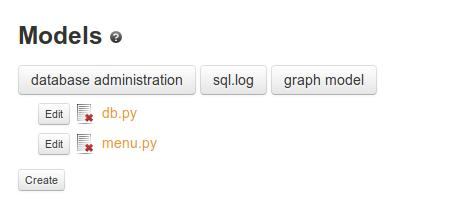
\includegraphics{src/img/models_menu.jpg}
\caption{Menú Modelos}
\end{figure}

\textbf{\emph{web2py}} se encarga de crear las tablas necesarias en la
base de datos que le hayamos indicado que use.

Al crear la aplicación \_\textbf{web2py} ha creado en la base de datos
todas las tablas relacionadas con la gestión de usuarios y sus
privilegios.

Si echamos un ojo al modelo gráfico (\emph{Graphs Models}) veremos las
tablas que \textbf{\emph{web2py}} ha creado por defecto y las relaciones
entre ellas.

Si vemos el log de comandos de sql (\emph{sql.log}) veremos los comandos
que \textbf{\emph{web2py}} ha ejecutado en el motor de base de datos.

Y por último si vemos \emph{database administration} podremos ver las
tablas creadas en la base de datos, e incluso crear nuevos registros en
esas tablas.

También podemos echar un ojo al contenido del fichero \texttt{db.py} o
\texttt{menu.py} pero por el momento \textbf{no} vamos a modificar nada
en esos ficheros.

\hypertarget{secciones-en-el-futuro}{%
\section{Secciones en el futuro}\label{secciones-en-el-futuro}}

\hypertarget{web2py-y-git}{%
\subsection{web2py y git}\label{web2py-y-git}}

\hypertarget{instalaciuxf3n-con-nginx}{%
\subsection{Instalación con nginx}\label{instalaciuxf3n-con-nginx}}

\hypertarget{certificados-lets-encrypt}{%
\subsection{Certificados let's
encrypt}\label{certificados-lets-encrypt}}

\end{document}
